\documentclass{article}

% TODO: please download neurips_2020.sty 
% from https://media.neurips.cc/Conferences/NeurIPS2020/Styles/neurips_2020.sty
% before building this document
\usepackage[preprint]{neurips_2020}

\usepackage[utf8]{inputenc} % allow utf-8 input
\usepackage[T1]{fontenc}    % use 8-bit T1 fonts
\usepackage{hyperref}       % hyperlinks
\usepackage{url}            % simple URL typesetting
\usepackage{booktabs}       % professional-quality tables
\usepackage{amsfonts}       % blackboard math symbols
\usepackage{nicefrac}       % compact symbols for 1/2, etc.
\usepackage{microtype}      % microtypography
\usepackage{graphicx}
\usepackage{amsthm}
\usepackage{amsmath}
\usepackage{bbm}
\usepackage{subfigure}

\newtheorem{theorem}{Theorem}

\title{Spectral clustering}

% The \author macro works with any number of authors. There are two commands
% used to separate the names and addresses of multiple authors: \And and \AND.
%
% Using \And between authors leaves it to LaTeX to determine where to break the
% lines. Using \AND forces a line break at that point. So, if LaTeX puts 3 of 4
% authors names on the first line, and the last on the second line, try using
% \AND instead of \And before the third author name.

\author{%
  Davide Riva \\
  \texttt{driva95@protonmail.com}
}

\begin{document}

\maketitle

\begin{abstract}
    The term "spectral clustering" refers to a series of unsupervised techniques to perform community detection in graphs using eigenvalues and eigenvectors.
    Even though there are some review articles about it, they usually have a lack of empirical analyses linked to the theoretical proofs.
    In this document, we are going to cover that part through experiments.
\end{abstract}

\section{Introduction}
Spectral clustering identifies communities inside a graph.
In Section \ref{section:twocom} we analyse how to extract communities in a noiseless scenario
in which there is only one connected component identified as the only one community in the graph.
Then, Section \ref{section:multiplecom} considers multiple connected components and
Section \ref{section:noisecom} extends the previous ideas to a graph in which
the number of clusters is greater than the number of connected components.
Finally, Section \ref{section:nograph} explains how to use these techniques with data
which is not structured as a graph.

Note that every time we use the term "graph" we refer to undirected, weighted graphs
to avoid useless redundancy. All weights must be positive.

The experiments are written in Python in the form of Jupyter Notebooks
and they are provide together with this document as appendices.
The name of the used libraries and their version are also supplied through a \path{requirements.txt} file.

\section{Graphs with 1 connected component} \label{section:twocom}
We start by looking at a graph with a single connected component, as the one in Figure \ref{figure:plotga}.
We denote its weight matrix as $W \in \mathbb{R}^{n \times n}$.

\begin{figure}[hb]
    \hfill
    \subfigure[A graph with one connected component.]{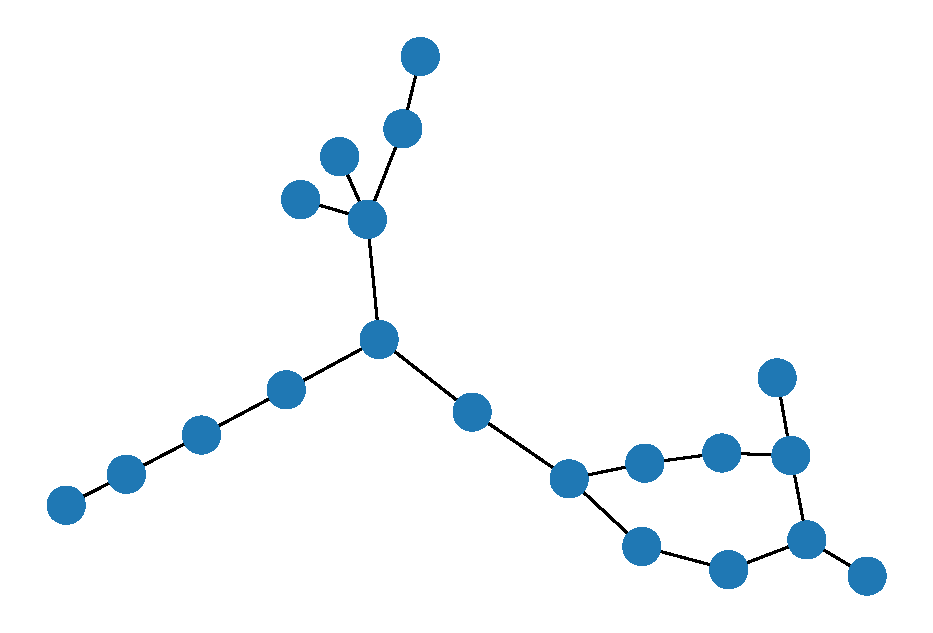
\includegraphics[width=0.5\textwidth]{figures/one-component.eps}}%
    \hfill
    \subfigure[A graph with three connected components.]{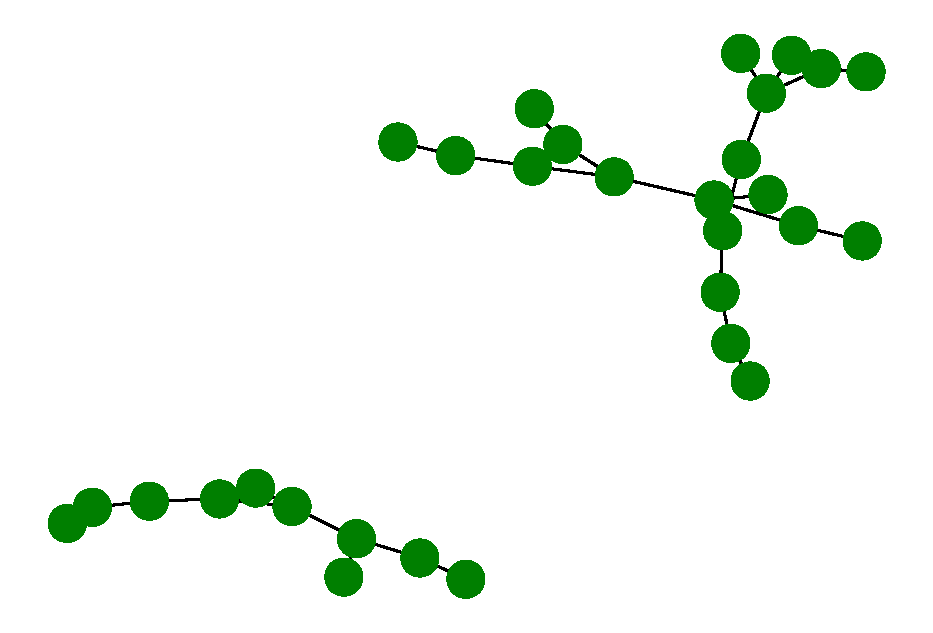
\includegraphics[width=0.5\textwidth]{figures/multiple-component.eps}}%
    \hfill
    \caption{Examples of graphs with various connected components.}%
    \label{figure:plotga}%
\end{figure}

The degree matrix $D$ of a graph is defined as a diagonal matrix whose diagonal elements are:
\begin{equation*}
    D_{ii} = \sum_{j=1}^n W_{ij}
\end{equation*}

The goal is to obtain an indicator vector $f = (f_1, \dots, f_n)$ which can identify which
node belongs to which connected component.
To do so, we build a matrix that we call Laplacian matrix:
\begin{equation*}
    L = D - W
\end{equation*}

\begin{theorem}
    Minimizing $\frac{1}{2} \sum_{i=1}^n \sum_{j=1}^n W_{ij} (f_i - f_j)$
    is equivalent to minimizing $f^T L f$.
\end{theorem}

\begin{proof}
    \begin{align*}
        f^T L f & = f^T D f - f^T W f                                                                                                 \\
                & = \sum_{i=1}^n D_{ii} f_i^2 - \sum_{i=1}^n \sum_{j=1}^n f_i f_j W_{ij}                                              \\
                & = \frac{1}{2} ( 2 \sum_{i=1}^n D_{ii} f_i^2 - 2 \sum_{i=1}^n \sum_{j=1}^n f_i f_j W_{ij})                           \\
                & = \frac{1}{2} ( \sum_{i=1}^n D_{ii} f_i^2 + \sum_{j=1}^n D_{jj} f_j^2 - 2 \sum_{i=1}^n \sum_{j=1}^n f_i f_j W_{ij}) \\
                & = \frac{1}{2} \sum_{i=1}^n \sum_{j=1}^n W_{ij} (f_i - f_j)^2 \tag*{\qedhere}
    \end{align*}
\end{proof}

We also know that $L$ is symmetric by definition. Furthermore, it is positive semi-definite since from the previous theorem
$f^T L f \geq 0 \; \forall f \in \mathbb{R}^n$.

It follows that the smallest eigenvalue of $L$ is 0. Its corresponding eigenvector is the vector $a [1, 1, \dots, 1], a \in \mathit{R}$
due to the fact that the sum of the elements of each row or column is always zero.
Note that if the graph has one connected component, the eigenvector corresponding to the eigenvalue with value 0 is the global minimum of the
minimization problem and a perfect solution for our task.

We can observe in an empirical way what we have just proved.
First, we generate a pre-defined number of graphs with one connected component.
In particular, each graph is a Watts–Strogatz model \cite{wc} which has the desired propriety of having a not small clustering coefficient.
Then, we produce a box plot of the values of each eigenvalue sorted in ascending order for each graph.
The resulting plot can be seen in Figure \ref{figure:oneeigen}.

\begin{figure}[ht]
    \centering
    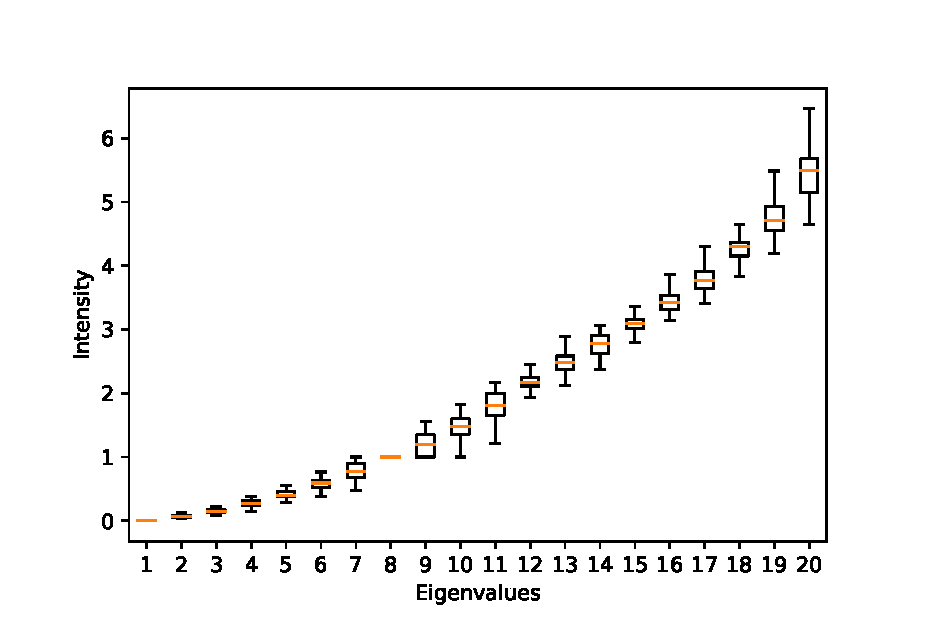
\includegraphics[width=0.5\linewidth]{figures/eigen-one-component.eps}
    \caption{Box plot of the eigenvalues of 100 graphs with 20 nodes and one connected component, sorted in ascending order for each graph.}
    \label{figure:oneeigen}
\end{figure}

\section{Graphs with multiple connected components} \label{section:multiplecom}
We now want to identify which node belongs to which connected component
when the graph has the number of connected components $k \geq 2$
as the one in Figure \ref{figure:plotga}.

First, we rearrange the matrix $L$ grouping together nodes in the same connected component.
In this way, $L$ is a block diagonal matrix with subgraphs $L_1, \dots, L_k$.
Now, each subgraph has one and only one connected component
and therefore it has one eigenvalue that is equal to zero,
as demonstrated in Section \ref{section:twocom}.

We also know from linear algebra that the set of eigenvalues of $L$
is composed of the eigenvalues of $L_1, \dots, L_k$.
Also, each corresponding eigenvector in $L_i$ is a valid eigenvector in $L$ with zero padding
in the other block positions.
It follows that the matrix $L$ has $k$ eigenvalues with value equals to zero and
one combination of eigenvalues valid in that eigenspace is composed of indicator vectors.
This propriety can be seen empirically in Figure \ref{figure:mcomp},
where each graph is again a Watts–Strogatz model.

\begin{figure}[hb]
    \hfill
    \subfigure[Graphs with two connected components.]{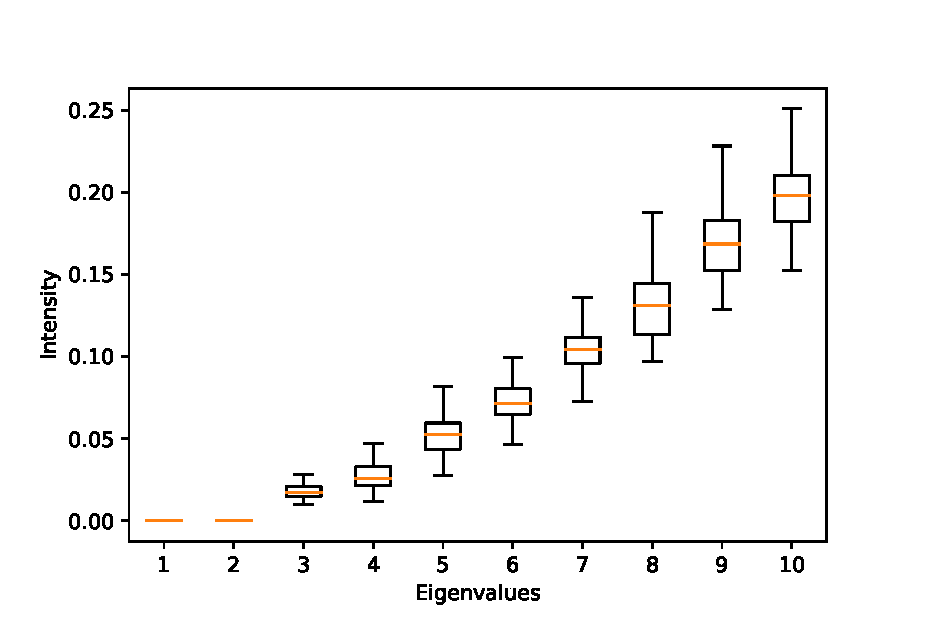
\includegraphics[width=0.3\textwidth]{figures/2-components.eps}}
    \hfill
    \subfigure[Graphs with four connected components.]{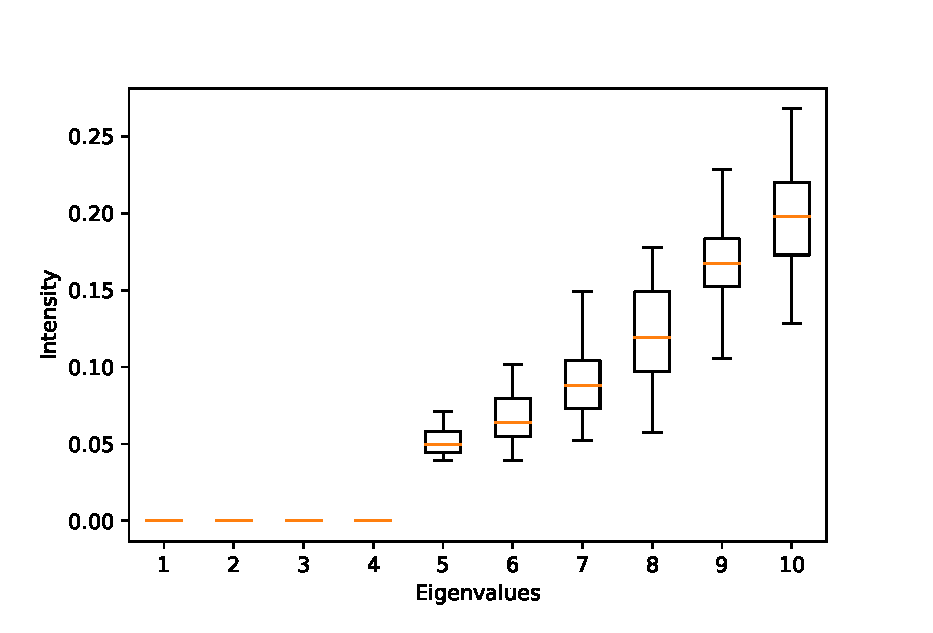
\includegraphics[width=0.3\textwidth]{figures/4-components.eps}}
    \hfill
    \subfigure[Graphs with eight connected components.]{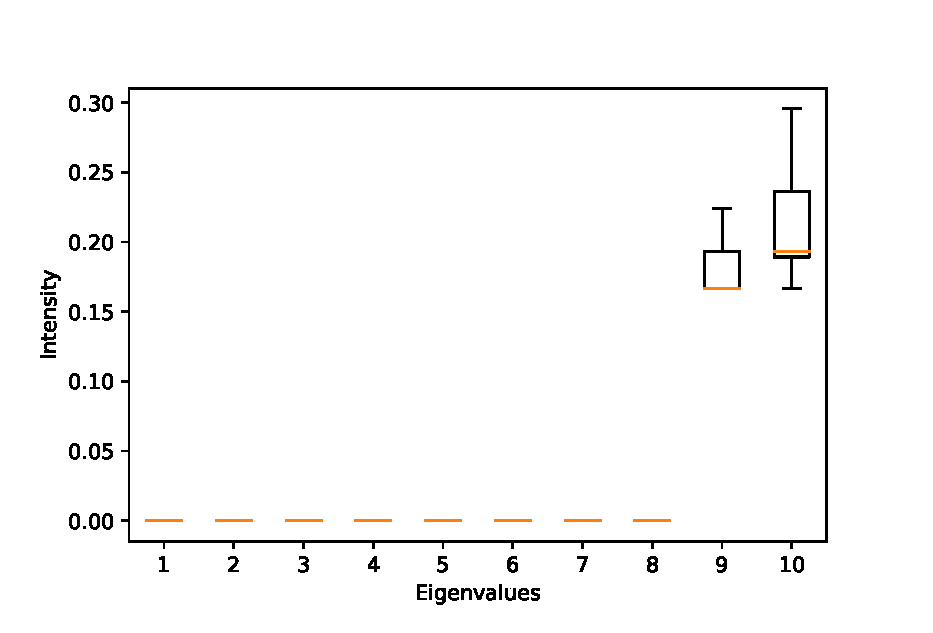
\includegraphics[width=0.3\textwidth]{figures/8-components.eps}}
    \hfill
    \label{figure:mcomp}
    \caption{Box plot of the first 10 eigenvalues of 100 graphs with 64 nodes and different connected components, sorted in ascending order for each graph.}
\end{figure}

Since in this scenario the eigenspace of the eigenvalues with value zero
is a linear combination of indicator vectors, we use them to identify the connected components.
In particular, we build a matrix $V \in \mathit{R}^{n \times k}$ where each column corresponds to
an eigenvector of the previous eigenspace.
Finally, K-means is performed over the matrix $V$ to group data due to the fact that groups in $V$
are linearly separable.

In order to see if the eigenvectors described before are good indicator vectors,
we build a graph with three connected components:
the first cluster corresponds to the first three nodes,
the second cluster is composed of the last two and the third has all the remaining ones.
Each connected component of the graph is a complete graph itself.
Figure \ref{figure:eivects} represents this configuration graphically.

\begin{figure}[hb]
    \hfill
    \subfigure{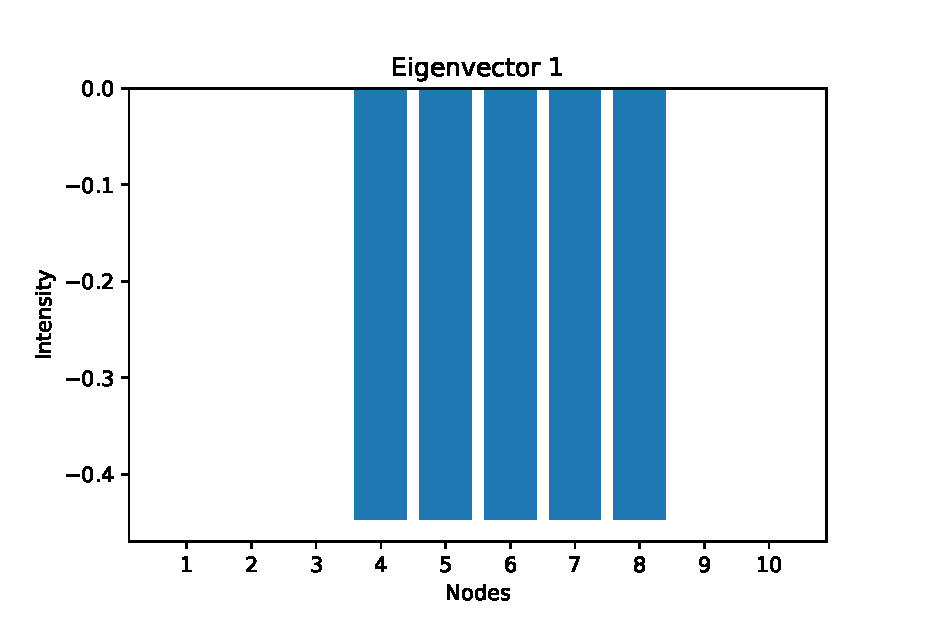
\includegraphics[width=0.3\textwidth]{figures/0-eigenvectors.eps}}%
    \hfill
    \subfigure{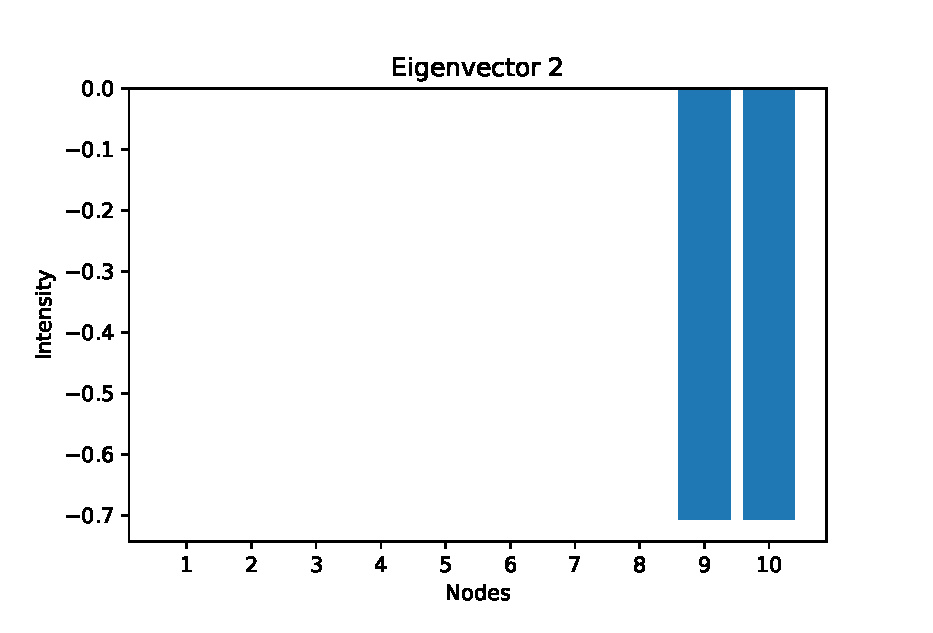
\includegraphics[width=0.3\textwidth]{figures/1-eigenvectors.eps}}%
    \hfill
    \subfigure{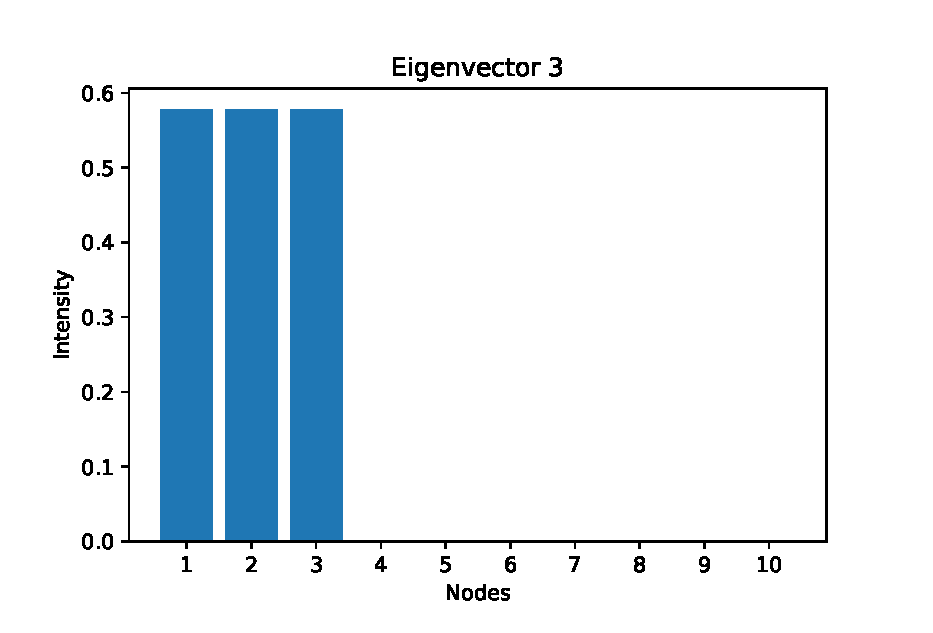
\includegraphics[width=0.3\textwidth]{figures/2-eigenvectors.eps}}%
    \hfill
    \caption{Example of eigenvectors used as indicator vectors.}%
    \label{figure:eivects}%
\end{figure}

\section{Considerations about noise} \label{section:noisecom}
Until now we considered the situation in which each detected community
corresponds to a connected component of the graph.

If we instead assume that each cluster is a tightly coupled group of nodes
with a low number of inter-community edges, we can treat these edges as noise added
to the situations described in the previous sections.
Given the noiseless adjacency matrix $A$,
we can view the edges presented before as a perturbation $H$ that produces the final
matrix $W = A + H$.

Thanks to the Davis–Kahan theorem \cite{davis1970rotation} we can state that small perturbations
in the Laplacian matrix lead to small perturbations in its eigenvectors and eigenvalues.
This means that if the noise (in our case, the addition of unwanted edges) is small,
it is still possible to perform spectral clustering.
In particular, we choose the number of communities looking at each eigengap:
small eigengaps are considered produced by noise,
while the first eigengap greater than the previous ones is assumed to be the dividing
indicator between eigenvectors used as indicator vectors and other eigenvectors.
Using the eigengap as a criterion to decide the number of communities in a graph
can be justified in other ways, well documented in \cite{DBLP:journals/corr/abs-0711-0189}.

To empirically verify the quality of using the eigengap to identify the number of clusters,
we start from a graph composed of three connected components which are complete graphs themselves and
we add iteratively more edges until all nodes are connected to everyone else.
As we can see from Figure \ref{figure:addingnoise}:
\begin{itemize}
    \item The smallest eigenvalue is zero all the time since there is always at least one connected component in a graph.
    \item The first three eigenvalues in ascending order are initially zero when there is no noise and then they grow when edges are added.
    \item The eigengap between the third and the fourth eigenvalue is bigger than the others until there is too much noise.
\end{itemize}

\begin{figure}[ht]
    \centering
    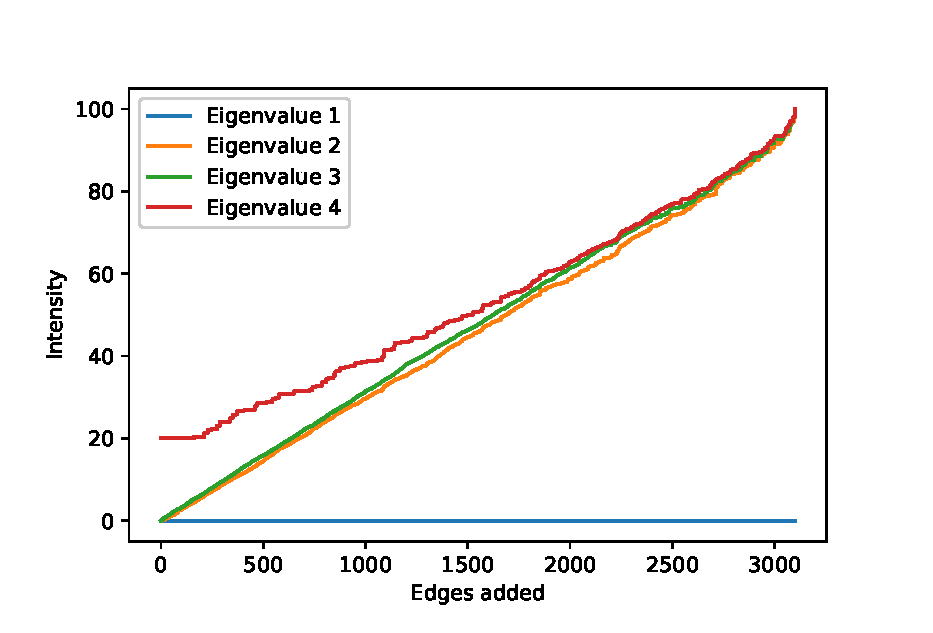
\includegraphics[width=0.5\linewidth]{figures/adding-noise.eps}
    \caption{Example of the effect of noise in the eigenvalues intensities in a graph with 3 connected components.}
    \label{figure:addingnoise}
\end{figure}


\section{EE} \label{section:nograph}
\dots

\pagebreak
\nocite{*}
\bibliography{references}
\bibliographystyle{plain}

\pagebreak
\section{Submission of papers to NeurIPS 2020}

NeurIPS requires electronic submissions.  The electronic submission site is
\begin{center}
    \url{https://cmt3.research.microsoft.com/NeurIPS2020/}
\end{center}

Please read the instructions below carefully and follow them faithfully.

\subsection{Style}

Papers to be submitted to NeurIPS 2020 must be prepared according to the
instructions presented here. Papers may only be up to eight pages long,
including figures. Additional pages \emph{containing only a section on the broader impact, acknowledgments and/or cited references} are allowed. Papers that exceed eight pages of content will not be reviewed, or in any other way considered for
presentation at the conference.

The margins in 2020 are the same as those in 2007, which allow for $\sim$$15\%$
more words in the paper compared to earlier years.

Authors are required to use the NeurIPS \LaTeX{} style files obtainable at the
NeurIPS website as indicated below. Please make sure you use the current files
and not previous versions. Tweaking the style files may be grounds for
rejection.

\subsection{Retrieval of style files}

The style files for NeurIPS and other conference information are available on
the World Wide Web at
\begin{center}
    \url{http://www.neurips.cc/}
\end{center}
The file \verb+neurips_2020.pdf+ contains these instructions and illustrates the
various formatting requirements your NeurIPS paper must satisfy.

The only supported style file for NeurIPS 2020 is \verb+neurips_2020.sty+,
rewritten for \LaTeXe{}.  \textbf{Previous style files for \LaTeX{} 2.09,
    Microsoft Word, and RTF are no longer supported!}

The \LaTeX{} style file contains three optional arguments: \verb+final+, which
creates a camera-ready copy, \verb+preprint+, which creates a preprint for
submission to, e.g., arXiv, and \verb+nonatbib+, which will not load the
\verb+natbib+ package for you in case of package clash.

\paragraph{Preprint option}
If you wish to post a preprint of your work online, e.g., on arXiv, using the
NeurIPS style, please use the \verb+preprint+ option. This will create a
nonanonymized version of your work with the text ``Preprint. Work in progress.''
in the footer. This version may be distributed as you see fit. Please \textbf{do
    not} use the \verb+final+ option, which should \textbf{only} be used for
papers accepted to NeurIPS.

At submission time, please omit the \verb+final+ and \verb+preprint+
options. This will anonymize your submission and add line numbers to aid
review. Please do \emph{not} refer to these line numbers in your paper as they
will be removed during generation of camera-ready copies.

The file \verb+neurips_2020.tex+ may be used as a ``shell'' for writing your
paper. All you have to do is replace the author, title, abstract, and text of
the paper with your own.

The formatting instructions contained in these style files are summarized in
Sections \ref{gen_inst}, \ref{headings}, and \ref{others} below.

\section{General formatting instructions}
\label{gen_inst}

The text must be confined within a rectangle 5.5~inches (33~picas) wide and
9~inches (54~picas) long. The left margin is 1.5~inch (9~picas).  Use 10~point
type with a vertical spacing (leading) of 11~points.  Times New Roman is the
preferred typeface throughout, and will be selected for you by default.
Paragraphs are separated by \nicefrac{1}{2}~line space (5.5 points), with no
indentation.

The paper title should be 17~point, initial caps/lower case, bold, centered
between two horizontal rules. The top rule should be 4~points thick and the
bottom rule should be 1~point thick. Allow \nicefrac{1}{4}~inch space above and
below the title to rules. All pages should start at 1~inch (6~picas) from the
top of the page.

For the final version, authors' names are set in boldface, and each name is
centered above the corresponding address. The lead author's name is to be listed
first (left-most), and the co-authors' names (if different address) are set to
follow. If there is only one co-author, list both author and co-author side by
side.

Please pay special attention to the instructions in Section \ref{others}
regarding figures, tables, acknowledgments, and references.

\section{Headings: first level}
\label{headings}

All headings should be lower case (except for first word and proper nouns),
flush left, and bold.

First-level headings should be in 12-point type.

\subsection{Headings: second level}

Second-level headings should be in 10-point type.

\subsubsection{Headings: third level}

Third-level headings should be in 10-point type.

\paragraph{Paragraphs}

There is also a \verb+\paragraph+ command available, which sets the heading in
bold, flush left, and inline with the text, with the heading followed by 1\,em
of space.

\section{Citations, figures, tables, references}
\label{others}

These instructions apply to everyone.

\subsection{Citations within the text}

The \verb+natbib+ package will be loaded for you by default.  Citations may be
author/year or numeric, as long as you maintain internal consistency.  As to the
format of the references themselves, any style is acceptable as long as it is
used consistently.

The documentation for \verb+natbib+ may be found at
\begin{center}
    \url{http://mirrors.ctan.org/macros/latex/contrib/natbib/natnotes.pdf}
\end{center}
Of note is the command \verb+\citet+, which produces citations appropriate for
use in inline text.  For example,
\begin{verbatim}
   \citet{hasselmo} investigated\dots
\end{verbatim}
produces
\begin{quote}
    Hasselmo, et al.\ (1995) investigated\dots
\end{quote}

If you wish to load the \verb+natbib+ package with options, you may add the
following before loading the \verb+neurips_2020+ package:
\begin{verbatim}
   \PassOptionsToPackage{options}{natbib}
\end{verbatim}

If \verb+natbib+ clashes with another package you load, you can add the optional
argument \verb+nonatbib+ when loading the style file:
\begin{verbatim}
   \usepackage[nonatbib]{neurips_2020}
\end{verbatim}

As submission is double blind, refer to your own published work in the third
person. That is, use ``In the previous work of Jones et al.\ [4],'' not ``In our
previous work [4].'' If you cite your other papers that are not widely available
(e.g., a journal paper under review), use anonymous author names in the
citation, e.g., an author of the form ``A.\ Anonymous.''

\subsection{Footnotes}

Footnotes should be used sparingly.  If you do require a footnote, indicate
footnotes with a number\footnote{Sample of the first footnote.} in the
text. Place the footnotes at the bottom of the page on which they appear.
Precede the footnote with a horizontal rule of 2~inches (12~picas).

Note that footnotes are properly typeset \emph{after} punctuation
marks.\footnote{As in this example.}

\subsection{Figures}

\begin{figure}
    \centering
    \fbox{\rule[-.5cm]{0cm}{4cm} \rule[-.5cm]{4cm}{0cm}}
    \caption{Sample figure caption.}
\end{figure}

All artwork must be neat, clean, and legible. Lines should be dark enough for
purposes of reproduction. The figure number and caption always appear after the
figure. Place one line space before the figure caption and one line space after
the figure. The figure caption should be lower case (except for first word and
proper nouns); figures are numbered consecutively.

You may use color figures.  However, it is best for the figure captions and the
paper body to be legible if the paper is printed in either black/white or in
color.

\subsection{Tables}

All tables must be centered, neat, clean and legible.  The table number and
title always appear before the table.  See Table~\ref{sample-table}.

Place one line space before the table title, one line space after the
table title, and one line space after the table. The table title must
be lower case (except for first word and proper nouns); tables are
numbered consecutively.

Note that publication-quality tables \emph{do not contain vertical rules.} We
strongly suggest the use of the \verb+booktabs+ package, which allows for
typesetting high-quality, professional tables:
\begin{center}
    \url{https://www.ctan.org/pkg/booktabs}
\end{center}
This package was used to typeset Table~\ref{sample-table}.

\begin{table}
    \caption{Sample table title}
    \label{sample-table}
    \centering
    \begin{tabular}{lll}
        \toprule
        \multicolumn{2}{c}{Part}                   \\
        \cmidrule(r){1-2}
        Name     & Description     & Size ($\mu$m) \\
        \midrule
        Dendrite & Input terminal  & $\sim$100     \\
        Axon     & Output terminal & $\sim$10      \\
        Soma     & Cell body       & up to $10^6$  \\
        \bottomrule
    \end{tabular}
\end{table}

\section{Final instructions}

Do not change any aspects of the formatting parameters in the style files.  In
particular, do not modify the width or length of the rectangle the text should
fit into, and do not change font sizes (except perhaps in the
\textbf{References} section; see below). Please note that pages should be
numbered.

\section{Preparing PDF files}

Please prepare submission files with paper size ``US Letter,'' and not, for
example, ``A4.''

Fonts were the main cause of problems in the past years. Your PDF file must only
contain Type 1 or Embedded TrueType fonts. Here are a few instructions to
achieve this.

\begin{itemize}

    \item You should directly generate PDF files using \verb+pdflatex+.

    \item You can check which fonts a PDF files uses.  In Acrobat Reader, select the
          menu Files$>$Document Properties$>$Fonts and select Show All Fonts. You can
          also use the program \verb+pdffonts+ which comes with \verb+xpdf+ and is
          available out-of-the-box on most Linux machines.

    \item The IEEE has recommendations for generating PDF files whose fonts are also
          acceptable for NeurIPS. Please see
          \url{http://www.emfield.org/icuwb2010/downloads/IEEE-PDF-SpecV32.pdf}

    \item \verb+xfig+ "patterned" shapes are implemented with bitmap fonts.  Use
          "solid" shapes instead.

    \item The \verb+\bbold+ package almost always uses bitmap fonts.  You should use
          the equivalent AMS Fonts:
          \begin{verbatim}
   \usepackage{amsfonts}
\end{verbatim}
          followed by, e.g., \verb+\mathbb{R}+, \verb+\mathbb{N}+, or \verb+\mathbb{C}+
          for $\mathbb{R}$, $\mathbb{N}$ or $\mathbb{C}$.  You can also use the following
          workaround for reals, natural and complex:
          \begin{verbatim}
   \newcommand{\RR}{I\!\!R} %real numbers
   \newcommand{\Nat}{I\!\!N} %natural numbers
   \newcommand{\CC}{I\!\!\!\!C} %complex numbers
\end{verbatim}
          Note that \verb+amsfonts+ is automatically loaded by the \verb+amssymb+ package.

\end{itemize}

If your file contains type 3 fonts or non embedded TrueType fonts, we will ask
you to fix it.

\subsection{Margins in \LaTeX{}}

Most of the margin problems come from figures positioned by hand using
\verb+\special+ or other commands. We suggest using the command
\verb+\includegraphics+ from the \verb+graphicx+ package. Always specify the
figure width as a multiple of the line width as in the example below:
\begin{verbatim}
   \usepackage[pdftex]{graphicx} ...
   \includegraphics[width=0.8\linewidth]{myfile.pdf}
\end{verbatim}
See Section 4.4 in the graphics bundle documentation
(\url{http://mirrors.ctan.org/macros/latex/required/graphics/grfguide.pdf})

A number of width problems arise when \LaTeX{} cannot properly hyphenate a
line. Please give LaTeX hyphenation hints using the \verb+\-+ command when
necessary.


\section*{Broader Impact}

Authors are required to include a statement of the broader impact of their work, including its ethical aspects and future societal consequences.
Authors should discuss both positive and negative outcomes, if any. For instance, authors should discuss a)
who may benefit from this research, b) who may be put at disadvantage from this research, c) what are the consequences of failure of the system, and d) whether the task/method leverages
biases in the data. If authors believe this is not applicable to them, authors can simply state this.

Use unnumbered first level headings for this section, which should go at the end of the paper. {\bf Note that this section does not count towards the eight pages of content that are allowed.}

\begin{ack}
    Use unnumbered first level headings for the acknowledgments. All acknowledgments
    go at the end of the paper before the list of references. Moreover, you are required to declare
    funding (financial activities supporting the submitted work) and competing interests (related financial activities outside the submitted work).
    More information about this disclosure can be found at: \url{https://neurips.cc/Conferences/2020/PaperInformation/FundingDisclosure}.


    Do {\bf not} include this section in the anonymized submission, only in the final paper. You can use the \texttt{ack} environment provided in the style file to autmoatically hide this section in the anonymized submission.
\end{ack}
\end{document}